\phant{KẾT QUẢ VÀ PHÂN TÍCH}\label{sec:ketqua}

\subsection{Tổng quan tỉ lệ thành công}

Bảng~\ref{tab:success} trình bày tỉ lệ thành công của bốn mô hình trên toàn bộ
năm biến thể. Đây là bảng tổng hợp trung tâm của bài báo: nó cho thấy khoảng cách
lớn giữa “biên dịch được” và “chạy đúng”, đồng thời cho thấy không có mô hình nào
đạt kết quả hoàn hảo ngoài ChatGPT-5.

\begin{table}[H]
\centering
\small
\caption{Tỉ lệ thành công trên toàn bộ năm biến thể: số gốc ở Bảng~III của bài báo
\cite{diehl2026} đặt cạnh kết quả tính lại từ Bảng~I--II (dựng chi tiết ở
Bảng~\ref{tab:detail}).}
\label{tab:success}
\begin{tabular}{@{}lcccc@{}}
\toprule
\textbf{Tiêu chí} & \textbf{ChatGPT-5} & \textbf{ChatGPT-4} & \textbf{Claude} & \textbf{LLaMA} \\
\midrule
Biên dịch & 100\% (5/5) & 100\% (5/5) & 100\% (5/5) & 40\% / 60\% (3/5)$^*$ \\
Thực thi  & 100\% (5/5) & 20\% (1/5)  & 40\% / 60\% (3/5)$^*$ & 0\% (0/5)$^\dagger$ \\
Tính đúng & 100\% (5/5) & 100\% (5/5) & 100\% (5/5) & 40\% / 60\% (3/5)$^*$ \\
\bottomrule
\end{tabular}
\par\vspace{4pt}
{\footnotesize\raggedright
$^*$ Số trước dấu ``/'' là giá trị in trong Bảng~III của bài báo gốc; số sau là
tỉ lệ tính trực tiếp từ 5 biến thể trong Bảng~I và Bảng~II gốc.
$^\dagger$ Bảng~III và Bảng~I--II đều ghi 0\% (0/5), trong khi phần văn bản
Mục~VI.C gốc nêu LLaMA thực thi thành công một chương trình (20\%).\par}
\end{table}

Ba quan sát rút ra từ bảng:

\begin{enumerate}
  \item \textbf{Cú pháp không phải rào cản chính.} Ba trong bốn mô hình biên dịch
        100\% (5/5) chương trình. Ngay cả LLaMA, mô hình yếu nhất, cũng đạt 40\%
        theo Bảng~III gốc và 60\% (3/5: bất đồng bộ, OpenMP, MPI+OpenMP) nếu tính
        từ Bảng~I--II — nghĩa là phần lớn lỗi không nằm ở cú pháp C++ mà ở ngữ
        nghĩa song song và kiến thức hệ sinh thái.
  \item \textbf{Thực thi là điểm rơi lớn nhất.} ChatGPT-4 biên dịch 100\% nhưng
        chỉ 20\% (1/5, duy nhất MPI+OpenMP) chạy không lỗi; Claude đạt 40\% theo
        Bảng~III gốc (3/5 = 60\% theo Bảng~I--II); LLaMA đạt 0\% (0/5) theo các
        bảng tổng hợp. Đây là bằng chứng định lượng cho luận điểm: mã song song có
        thể “trông đúng” mà vẫn sai ở tầng điều khiển luồng, vòng đời tài nguyên
        hoặc định dạng đầu ra.
  \item \textbf{ChatGPT-5 là mô hình duy nhất đạt 100\% ở cả ba tiêu chí.} Điều
        đáng chú ý là nó không chỉ tránh lỗi mới mà còn sửa đúng các lỗi mà
        ChatGPT-4 mắc phải, cho thấy khả năng nắm bắt ngữ cảnh công cụ tốt hơn.
\end{enumerate}

\noindent\textit{Đối chiếu tính nhất quán của dữ liệu trong bài báo gốc.} Khi đối
chiếu xuyên suốt các bảng, hình vẽ và phần văn bản của \cite{diehl2026}, báo cáo
ghi nhận sáu điểm không nhất quán nội tại trong chính bài báo gốc và trình bày
minh bạch tại đây để người đọc tiện kiểm chứng:
\begin{itemize}
  \item \textbf{Bảng~III so với Bảng~I--II và Mục~VI.C:} Bảng~III ghi Claude (Thực
        thi), LLaMA (Biên dịch) và LLaMA (Tính đúng) đều là 40\%, trong khi
        Bảng~I--II đánh dấu đạt 3/5 biến thể (60\%) cho cả ba ô này; với LLaMA
        (Thực thi), Bảng~III và Bảng~I--II đều cho 0\% (0/5) nhưng văn bản
        Mục~VI.C viết “một chương trình (20\%)”.
  \item \textbf{Vị trí lỗi \code{std::distance} của LLaMA:} Mục~VI.A.4 mô tả lỗi
        biên dịch \code{std::distance} ở biến thể \emph{thuật toán song song}
        (khớp Bảng~I: bất đồng bộ \code{Build = \checkmark}, thuật toán song song
        \code{Build = $\times$}), nhưng Bảng~IV gốc lại xếp lỗi này vào dòng
        \emph{bất đồng bộ}.
  \item \textbf{Cơ chế đặt số luồng TBB:} Mục~VI.A.2 nêu đúng API
        \code{tbb::global\_control}, còn cột cách khắc phục ở Bảng~IV gốc lại ghi
        biến môi trường \code{TBB\_NUM\_THREADS} (không phải biến chuẩn của Intel
        TBB).
  \item \textbf{Số dòng thêm cho coroutine LLaMA:} Mục~VII gốc ghi thêm 39 dòng,
        trong khi chú thích Fig.~3 gốc ghi 37 dòng.
  \item \textbf{Số lõi trên một nút:} Mục~VI.A.1 gốc viết cần phóng lớn ảnh để mở
        rộng tới 24 lõi, nhưng cấu hình phần cứng ở Mục~VIII và toàn bộ đồ thị
        Fig.~6 gốc đều là 20 lõi/nút (Intel Xeon Gold 6148).
  \item \textbf{Ký hiệu đồ thị OpenMP (Fig.~6d):} Mục~VIII.A gốc kết luận mã
        OpenMP của ChatGPT-5 vượt các mã khác và mã con người, nhưng đường đạt
        $6\times 10^9$ trên Fig.~6(d) gốc lại mang ký hiệu ô vuông của ChatGPT-4.
\end{itemize}
Báo cáo giữ nguyên số liệu trích từ bài báo gốc tại các bảng tương ứng, đồng thời
lấy Bảng~I--II và phần mô tả phần cứng/đồ thị làm mốc đối chiếu để bảo đảm tính
nhất quán nội bộ.

\subsection{Bộ nhớ chia sẻ: lỗi theo từng mô hình}

\subsubsection{ChatGPT-4: phân tích dòng lệnh và backend}

Với cả bốn biến thể bộ nhớ chia sẻ, ChatGPT-4 in ra hướng dẫn dòng lệnh đầy đủ
như trong Đoạn mã~\ref{lst:usage}, nhưng chỉ phân tích tham số \code{-t}. Các
tham số còn lại — kích thước ảnh, số vòng lặp, tâm, tỉ lệ — bị bỏ qua và luôn
dùng giá trị mặc định.

\begin{lstlisting}[language={},caption={Hướng dẫn dòng lệnh do ChatGPT-4 sinh (Listing 1 trong bài báo gốc).},label={lst:usage},numbers=none,basicstyle=\ttfamily\small]
# Usage: [-t threads] [width height [max_iter [x_center y_center [scale]]]]
./exe -t 8 1920 1080 1000 -0.75 0.0 3.0
\end{lstlisting}

Đây là lỗi “đặc tả bề mặt”: chương trình \emph{trông} có giao diện cấu hình, in
ra hướng dẫn đúng, nhưng hành vi thực tế chỉ hỗ trợ một phần. Với phép đo mở rộng,
hệ quả là không thể tăng kích thước ảnh để tạo đủ tải cho 20 lõi (Mục~VI.A.1 gốc
ghi 24 lõi, nhưng phần cứng thực tế ở Bảng~\ref{tab:env} là 20 lõi/nút) nếu không
sửa mã. Nhóm tác giả phải thay đổi kích thước ảnh mặc định để phép đo có ý nghĩa.

Lỗi thứ hai tinh vi hơn. Mã thuật toán song song giả định GCC dùng OpenMP cho
\code{std::execution::par} và đặt biến môi trường \code{OPENMP\_NUM\_THREADS}
(nguyên văn theo bài báo gốc; tên biến chuẩn của OpenMP thực tế là
\code{OMP\_NUM\_THREADS}) để giới hạn số luồng. Thực tế, libstdc++ dùng Intel
TBB, nên biến này bị bỏ qua và chương trình luôn chạy trên toàn bộ lõi. Cách sửa
đúng là dùng API TBB, cụ thể \code{tbb::global\_control} với
\code{max\_allowed\_parallelism} như Mục~VI.A.2 của bài báo (lưu ý Bảng~IV gốc
nhắc \code{TBB\_NUM\_THREADS} nhưng biến này không tồn tại chuẩn trong TBB). Đây
không phải lỗi cú pháp; nó đòi hỏi kiến thức về backend của thư viện chuẩn trên
một trình biên dịch cụ thể.

\subsubsection{ChatGPT-5: không có lỗi}

ChatGPT-5 không gặp lỗi ở bất kỳ biến thể bộ nhớ chia sẻ nào. Đáng chú ý là nó
phân tích đầy đủ các tham số dòng lệnh — khắc phục lỗi của ChatGPT-4 — và dùng
đúng \code{tbb::global\_control} để giới hạn số luồng. Điều này cho thấy mô hình
không chỉ học cú pháp mà còn học được mẫu tích hợp giữa chuẩn C++ và backend cụ
thể.

\subsubsection{Claude: vòng đời coroutine và số luồng}

Toàn bộ mã của Claude biên dịch được và sau khi khắc phục lỗi đều cho ảnh kết quả
đúng. Tuy nhiên ở tầng thực thi (Bảng~\ref{tab:detail}), trong bốn biến thể bộ nhớ
chia sẻ chỉ có \emph{bất đồng bộ} và \emph{OpenMP} chạy đạt yêu cầu; hai biến thể
còn lại đều bị đánh dấu lỗi thực thi. Biến thể coroutine treo và không bao giờ kết
thúc. Nguyên nhân là vòng lặp chờ trong Đoạn mã~\ref{lst:corobug}: \code{done()}
không bao giờ trả về \code{true} vì coroutine dùng
\code{final\_suspend = std::suspend\_never}. Khi coroutine kết thúc, frame bị hủy
ngay; trạng thái “đã hoàn thành” không còn để quan sát (và truy cập handle sau khi
tự hủy là hành vi không xác định). Đổi sang \code{std::suspend\_always} khắc phục
được vấn đề.

Với thuật toán song song, mã sinh ra có một chú thích nhắc người dùng đặt số
luồng, như trong Đoạn mã~\ref{lst:comment}. Chú thích này đúng về mặt kỹ thuật,
nhưng bản thân chương trình không thực hiện việc đặt số luồng; nó chỉ ghi nhận
rằng việc đó là cần thiết. Đây là dạng lỗi “biết mà không làm”: mô hình hiểu vấn
đề nhưng không chuyển hiểu biết thành mã.

\begin{lstlisting}[language=C++,caption={Chú thích về số luồng trong mã Claude (Listing 3 trong bài báo gốc).},label={lst:comment}]
/* Set the number of threads for parallel execution
 * Note: C++17 parallel algorithms may not directly use this,
 * but some implementations respect thread pool sizes.
 */
\end{lstlisting}

\subsubsection{LLaMA: chuỗi lỗi chồng chất}

LLaMA là mô hình duy nhất gặp lỗi ở cả bốn biến thể bộ nhớ chia sẻ, và các lỗi có
tính chồng chất: sửa lỗi trước làm lộ lỗi sau.

\begin{itemize}
  \item \textbf{Bất đồng bộ}: chương trình cho ảnh đen với cả một luồng và nhiều
        luồng (lưu ý: Bảng~IV bài báo gốc còn xếp lỗi biên dịch
        \code{std::distance} với đối số \code{Pixel*} vào mục này, trong khi phần
        văn bản mục VI.A.4 lại mô tả lỗi đó ở biến thể thuật toán song song và
        Bảng~I đánh dấu bản bất đồng bộ biên dịch thành công).
  \item \textbf{Thuật toán song song}: hai lỗi biên dịch. Thứ nhất là lỗi
        \code{std::distance} khi truyền \code{Pixel*} thay vì iterator. Thứ hai
        là việc dùng \code{execution\_policy\_tag::concurrency\_hint = numThreads}
        trong khi \code{execution\_policy\_tag} không hề được khai báo — một API
        không tồn tại. Sau khi sửa, chương trình biên dịch nhưng luôn dùng toàn bộ
        luồng.
  \item \textbf{Coroutine}: ba lớp lỗi. Đầu tiên là promise mismatch: mã dùng
        \code{co\_return} nhưng \code{Task::promise\_type} thiếu
        \code{return\_void()}. Sau khi thêm, chương trình biên dịch nhưng
        segmentation fault do work item bị giải phóng hai lần — một lần bởi
        \code{final\_suspend} và một lần bởi hàm hủy của \code{task}. Sau khi bỏ
        lần giải phóng thứ hai, chương trình chạy nhưng cho ảnh đen vì màu được
        tính theo P5 (8 bit) trong khi ảnh được ghi theo P4 (1 bit). Chỉ sau khi
        đổi định dạng, ảnh mới đúng.
  \item \textbf{OpenMP}: biên dịch được nhưng không tôn trọng số luồng; luôn chạy
        trên toàn bộ lõi hoặc số lõi đặt trước.
\end{itemize}

Chuỗi lỗi này minh họa rõ nhất luận điểm trung tâm của bài báo: lỗi nguy hiểm
nhất trong mã song song không phải lỗi cú pháp, mà là lỗi ngữ nghĩa chỉ biểu hiện
qua hành vi chạy — treo, crash, ảnh sai, hoặc hiệu năng không tăng.

\subsection{Bộ nhớ phân tán: lỗi theo từng mô hình}

Với MPI+OpenMP, bức tranh đơn giản hơn nhưng vẫn lộ ra các vấn đề đặc thù của
truyền thông.

\begin{itemize}
  \item \textbf{ChatGPT-4}: chương trình chạy không lỗi. Tuy nhiên, mã dùng lại
        cùng một hàm tô màu như bản bộ nhớ chia sẻ, không điều chỉnh theo ngữ
        cảnh phân tán. Đây là vấn đề nhất quán chất lượng, không phải lỗi chức
        năng.
  \item \textbf{ChatGPT-5}: biên dịch và chạy thành công, không gặp vấn đề nào.
  \item \textbf{Claude}: chạy đúng như kỳ vọng, không có lỗi.
  \item \textbf{LLaMA}: biên dịch được nhưng chỉ chạy đúng với một tiến trình. Với
        nhiều tiến trình, chương trình crash với \code{free(): invalid pointer};
        sau khi sửa, tiếp tục segmentation fault do lệch vùng đệm trong
        \code{MPI\_Gather}. Ngoài ra, mốc đo thời gian kết thúc được đặt trước
        bước gom dữ liệu, khiến thời gian truyền thông bị loại khỏi phép đo. Phải
        chỉnh lại mốc đo để so sánh công bằng với các mô hình khác.
\end{itemize}

Lỗi \code{MPI\_Gather} của LLaMA là ví dụ điển hình cho lớp lỗi biên: chương
trình không báo lỗi tại dòng gọi MPI, mà crash ở một điểm khác khi bộ nhớ đã bị
ghi đè. Việc tìm ra nguyên nhân đòi hỏi hiểu ngữ nghĩa tham số
\code{sendcount}/\code{recvcount} và kiểu dữ liệu của MPI, chứ không chỉ đọc thông
báo lỗi.

\subsection{Phân loại lỗi và mức độ khó}

Bảng~\ref{tab:errors} tổng hợp các lỗi tiêu biểu, nguyên nhân gốc và cách khắc
phục. Bảng~\ref{tab:taxonomy} phân loại theo tầng và mức độ khó.

\begin{table}[H]
\centering
\small
\caption{Tổng hợp lỗi tiêu biểu và cách khắc phục (tổng hợp từ Mục~VI và Bảng~IV
của bài báo gốc \cite{diehl2026}, khớp với Bảng~\ref{tab:detail}).}
\label{tab:errors}
\begin{tabularx}{\textwidth}{@{}p{1.9cm} p{2.3cm} X X@{}}
\toprule
\textbf{Mô hình} & \textbf{Biến thể} & \textbf{Lỗi quan sát} & \textbf{Cách khắc phục} \\
\midrule
ChatGPT-4 & 4 biến thể chia sẻ & Chỉ \code{-t} được phân tích; các tham số khác bị bỏ qua & Bổ sung phân tích dòng lệnh \\
ChatGPT-4 & Song song & Giả định GCC dùng OpenMP; đặt \code{OPENMP\_NUM\_THREADS} (chuẩn là \code{OMP\_NUM\_THREADS}) nhưng backend là TBB & Dùng \code{tbb::global\_control} \\
ChatGPT-5 & Tất cả (5 biến thể) & Không có lỗi & -- \\
Claude & Coroutine & Treo vì \code{done()} không bao giờ \code{true} do \code{final\_suspend = suspend\_never} & Đổi sang \code{suspend\_always} \\
Claude & Song song & Chỉ có chú thích nhắc đặt số luồng, không thực hiện & Đặt số luồng qua TBB \\
LLaMA & Bất đồng bộ & Ảnh đen (1 và nhiều luồng); bỏ qua \code{-t} (Bảng~IV gốc xếp lỗi \code{std::distance} vào mục này) & Sửa phần tính/ghi ảnh và đặt số luồng \\
LLaMA & Song song & Lỗi biên dịch \code{std::distance} (Mục~VI.A.4) và \code{execution\_policy\_tag} chưa khai báo; bỏ qua \code{-t} & Sửa kiểu iterator, bỏ biến không tồn tại \\
LLaMA & Coroutine & Promise mismatch; segfault do giải phóng hai lần; ảnh đen do P5 ghi vào P4; bỏ qua \code{-t} & Thêm \code{return\_void}, bỏ giải phóng thứ hai, đổi định dạng \\
LLaMA & OpenMP & Bỏ qua \code{-t}; luôn dùng toàn bộ hoặc số lõi đặt trước & Gán đúng số luồng OpenMP \\
LLaMA & MPI+OpenMP & \code{free(): invalid pointer}; segfault do lệch buffer \code{MPI\_Gather}; đo thời gian trước gather & Sửa cấp phát/buffer; chỉnh mốc đo \\
\bottomrule
\end{tabularx}
\end{table}

\begin{table}[H]
\centering
\small
\caption{Phân loại lỗi theo tầng, cách phát hiện và kiến thức cần có.}
\label{tab:taxonomy}
\begin{tabularx}{\textwidth}{@{}p{2.5cm} X p{3.1cm} p{2.2cm}@{}}
\toprule
\textbf{Tầng lỗi} & \textbf{Ví dụ quan sát} & \textbf{Cách phát hiện} & \textbf{Kiến thức cần} \\
\midrule
Cú pháp & \code{std::distance} sai kiểu; biến chưa khai báo & Trình biên dịch & C++ cơ bản \\
API / thư viện & \code{execution\_policy\_tag} không tồn tại; dùng \code{OPENMP\_NUM\_THREADS} cho TBB & Biên dịch hoặc đo số luồng & Hệ sinh thái, phiên bản thư viện \\
Ngữ nghĩa & \code{co\_return} thiếu \code{return\_void}; giải phóng hai lần & Crash, segfault, chạy sai & Vòng đời coroutine, quyền sở hữu \\
Đồng bộ / truyền thông & Lệch buffer \code{MPI\_Gather}; gom dữ liệu sai & Crash khi nhiều tiến trình & Ngữ nghĩa MPI, kích thước buffer \\
Định dạng dữ liệu & Tính màu P5 nhưng ghi P4 & Quan sát ảnh & Đặc tả Netpbm \\
Đo đạc & Kết thúc timer trước \code{MPI\_Gather} & So sánh đường cong bất thường & Phương pháp đo hiệu năng \\
\bottomrule
\end{tabularx}
\end{table}

Có thể xếp mức độ khó như sau. Lỗi cú pháp là dễ nhất: trình biên dịch chỉ đúng
dòng, người sửa chỉ cần biết C++ cơ bản. Lỗi API/thư viện khó hơn: chương trình
vẫn biên dịch, chỉ sai hành vi, nên phải biết backend nào đang chạy. Lỗi ngữ nghĩa
coroutine khó hơn nữa: phải hiểu \code{final\_suspend}, \code{promise\_type} và
quyền sở hữu frame. Lỗi truyền thông MPI khó nhất vì triệu chứng xuất hiện xa
nguyên nhân và phụ thuộc số tiến trình. Lỗi định dạng và lỗi đo đạc nằm ở giữa:
dễ phát hiện nếu có kiểm tra trực quan và so sánh đường cong, nhưng dễ bị bỏ qua
nếu chỉ tin vào “chương trình chạy không crash”.

\subsection{Chất lượng và chi phí mã nguồn}

Hình~\ref{fig:loc} trình bày số dòng mã do \code{cloc} đo được cho bốn biến thể
bộ nhớ chia sẻ. Nhìn chung, ChatGPT-5 và Claude sinh mã dài hơn ChatGPT-4 và
LLaMA. Chỉ với LLaMA, nhóm tác giả phải thêm một lượng đáng kể dòng mới để chương
trình coroutine hoạt động (Mục~VII gốc ghi 39 dòng, chú thích Fig.~3 gốc ghi 37
dòng); các mã còn lại chủ yếu sửa vài dòng hiện có.

\begin{figure}[H]
\centering
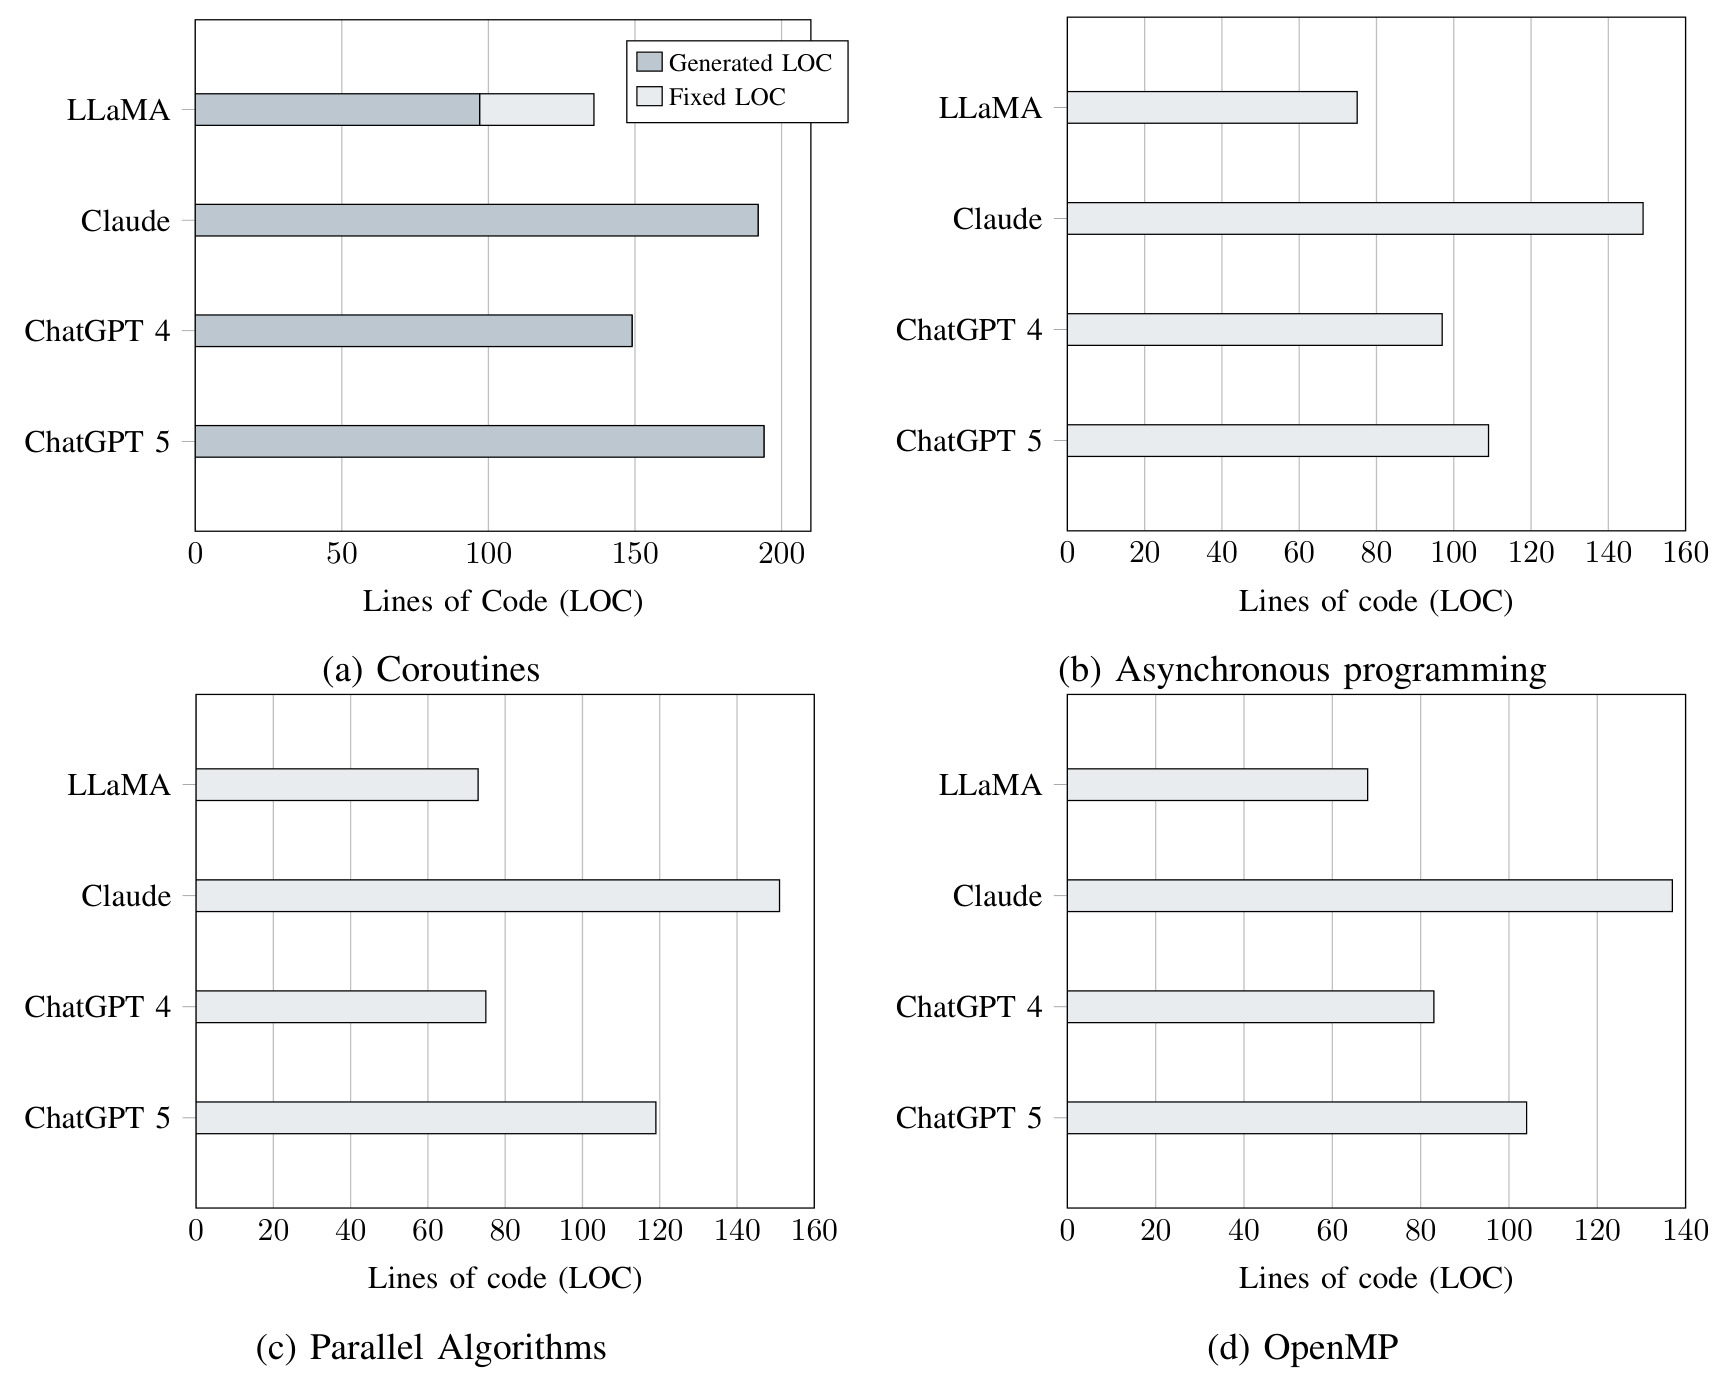
\includegraphics[width=0.92\textwidth]{figures/fig_loc.png}
\caption{Số dòng mã cho bốn biến thể bộ nhớ chia sẻ, trước và sau khi sửa.
Nguồn: bài báo \cite{diehl2026}.}
\label{fig:loc}
\end{figure}

Với bản phân tán, Bảng~\ref{tab:loc} cho thấy ChatGPT-5 sinh nhiều dòng nhất
(143), tiếp theo là Claude (116), ChatGPT-4 (91) và LLaMA (71, sau khi sửa thành
82). Việc phải thêm 11 dòng cho LLaMA cho thấy mã ngắn không đồng nghĩa với mã
tốt: mã càng ngắn càng có thể đã lược bỏ các bước kiểm tra cần thiết.

\begin{table}[H]
\centering
\small
\caption{Số dòng mã cho phiên bản MPI+OpenMP (Bảng V trong bài báo).}
\label{tab:loc}
\begin{tabular}{@{}lcccc@{}}
\toprule
\textbf{Mô hình} & \textbf{ChatGPT-5} & \textbf{ChatGPT-4} & \textbf{Claude} & \textbf{LLaMA} \\
\midrule
LOC & 143 & 91 & 116 & 71 $\to$ 82 \\
\bottomrule
\end{tabular}
\end{table}

Hình~\ref{fig:cocomo} biểu diễn chất lượng và công sức ước lượng theo COCOMO
(đơn vị tháng người, đi từ \term{Easy} bên trái sang \term{Difficult} bên phải).
Với bộ nhớ chia sẻ, ChatGPT-5 nằm ở góc trên--phải (“chất lượng cao nhất”, công
sức ước lượng tương đương hoặc hơi cao hơn nhẹ do số dòng mã dài hơn); Claude đứng
thứ hai; ChatGPT-4 thứ ba; LLaMA có hai ngoại lệ xấu ở coroutine và thuật toán
song song. Với bộ nhớ phân tán, ChatGPT-5 cũng có công sức ước lượng cao hơn do
số dòng nhiều hơn, còn LLaMA thấp nhất nhưng lại là mã duy nhất gặp lỗi thực thi.
Điều này củng cố nhận định: số dòng mã không tỉ lệ nghịch với chất lượng.

\begin{figure}[H]
\centering
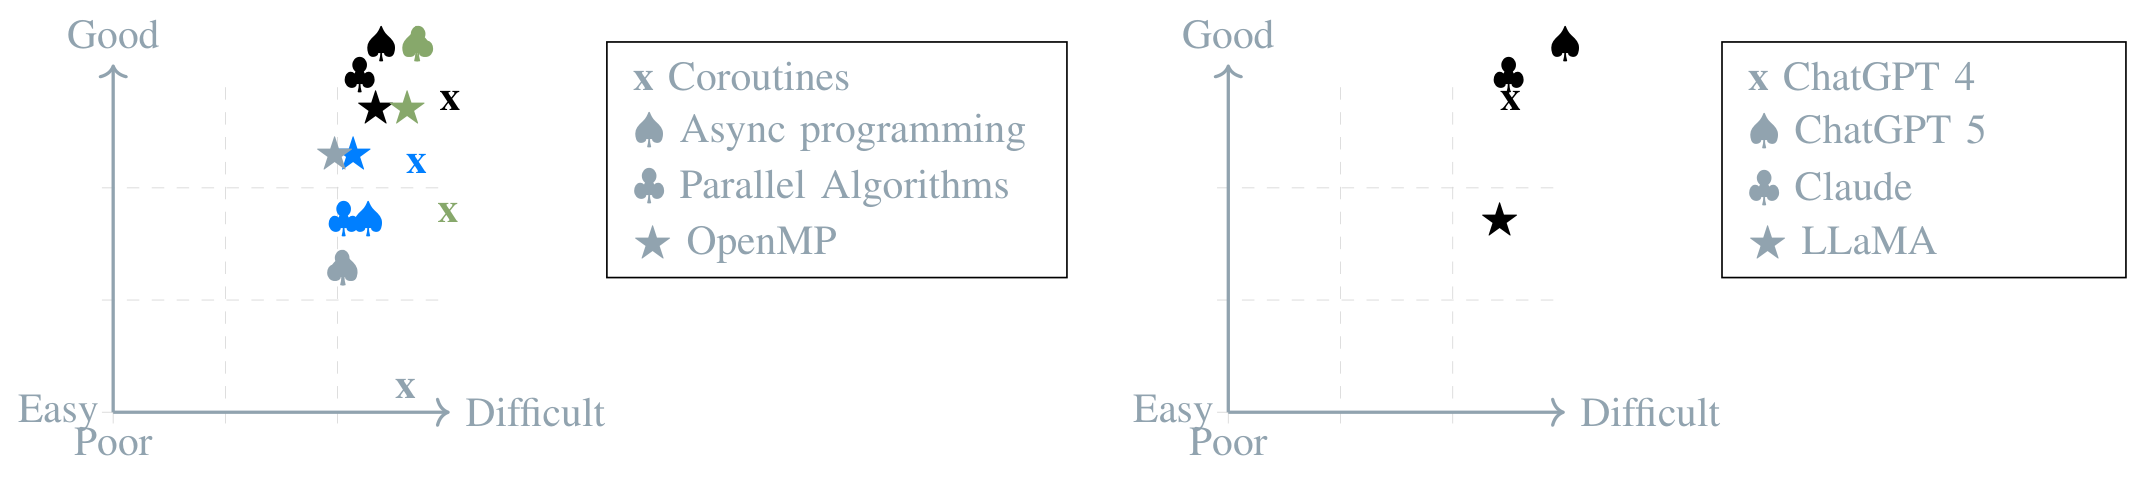
\includegraphics[width=0.98\textwidth]{figures/fig_cocomo.png}
\caption{Chất lượng (trục dọc, \term{Poor} $\to$ \term{Good}) và công sức ước
lượng theo COCOMO (trục ngang, \term{Easy} $\to$ \term{Difficult}) cho mã bộ nhớ
chia sẻ (trái) và phân tán (phải). Ở đồ thị trái, màu đen là ChatGPT-5, xanh dương
là ChatGPT-4, xanh lá là Claude và xám là LLaMA. Nguồn: bài báo \cite{diehl2026}.}
\label{fig:cocomo}
\end{figure}

Cần nhấn mạnh giới hạn của COCOMO: mô hình này được xây dựng cho phần mềm tuần
tự, không tính đến chi phí đồng bộ, truyền thông hay gỡ lỗi song song. Vì vậy,
các điểm trên Hình~\ref{fig:cocomo} chỉ nên dùng để so sánh tương đối giữa các
chương trình cùng loại, không nên diễn giải như dự báo nỗ lực tuyệt đối.

\subsection{Khả năng mở rộng trên một nút}

Hình~\ref{fig:scaling} trình bày kết quả mở rộng mạnh trên một nút (tối đa 20
lõi) cho bốn biến thể bộ nhớ chia sẻ. Trục dọc là số cập nhật điểm ảnh mỗi giây
(theo thang tuyến tính), trục ngang là số lõi. Đường màu xanh (ký hiệu trái tim)
là mã do con người viết, dùng làm tham chiếu.

\begin{figure}[H]
\centering
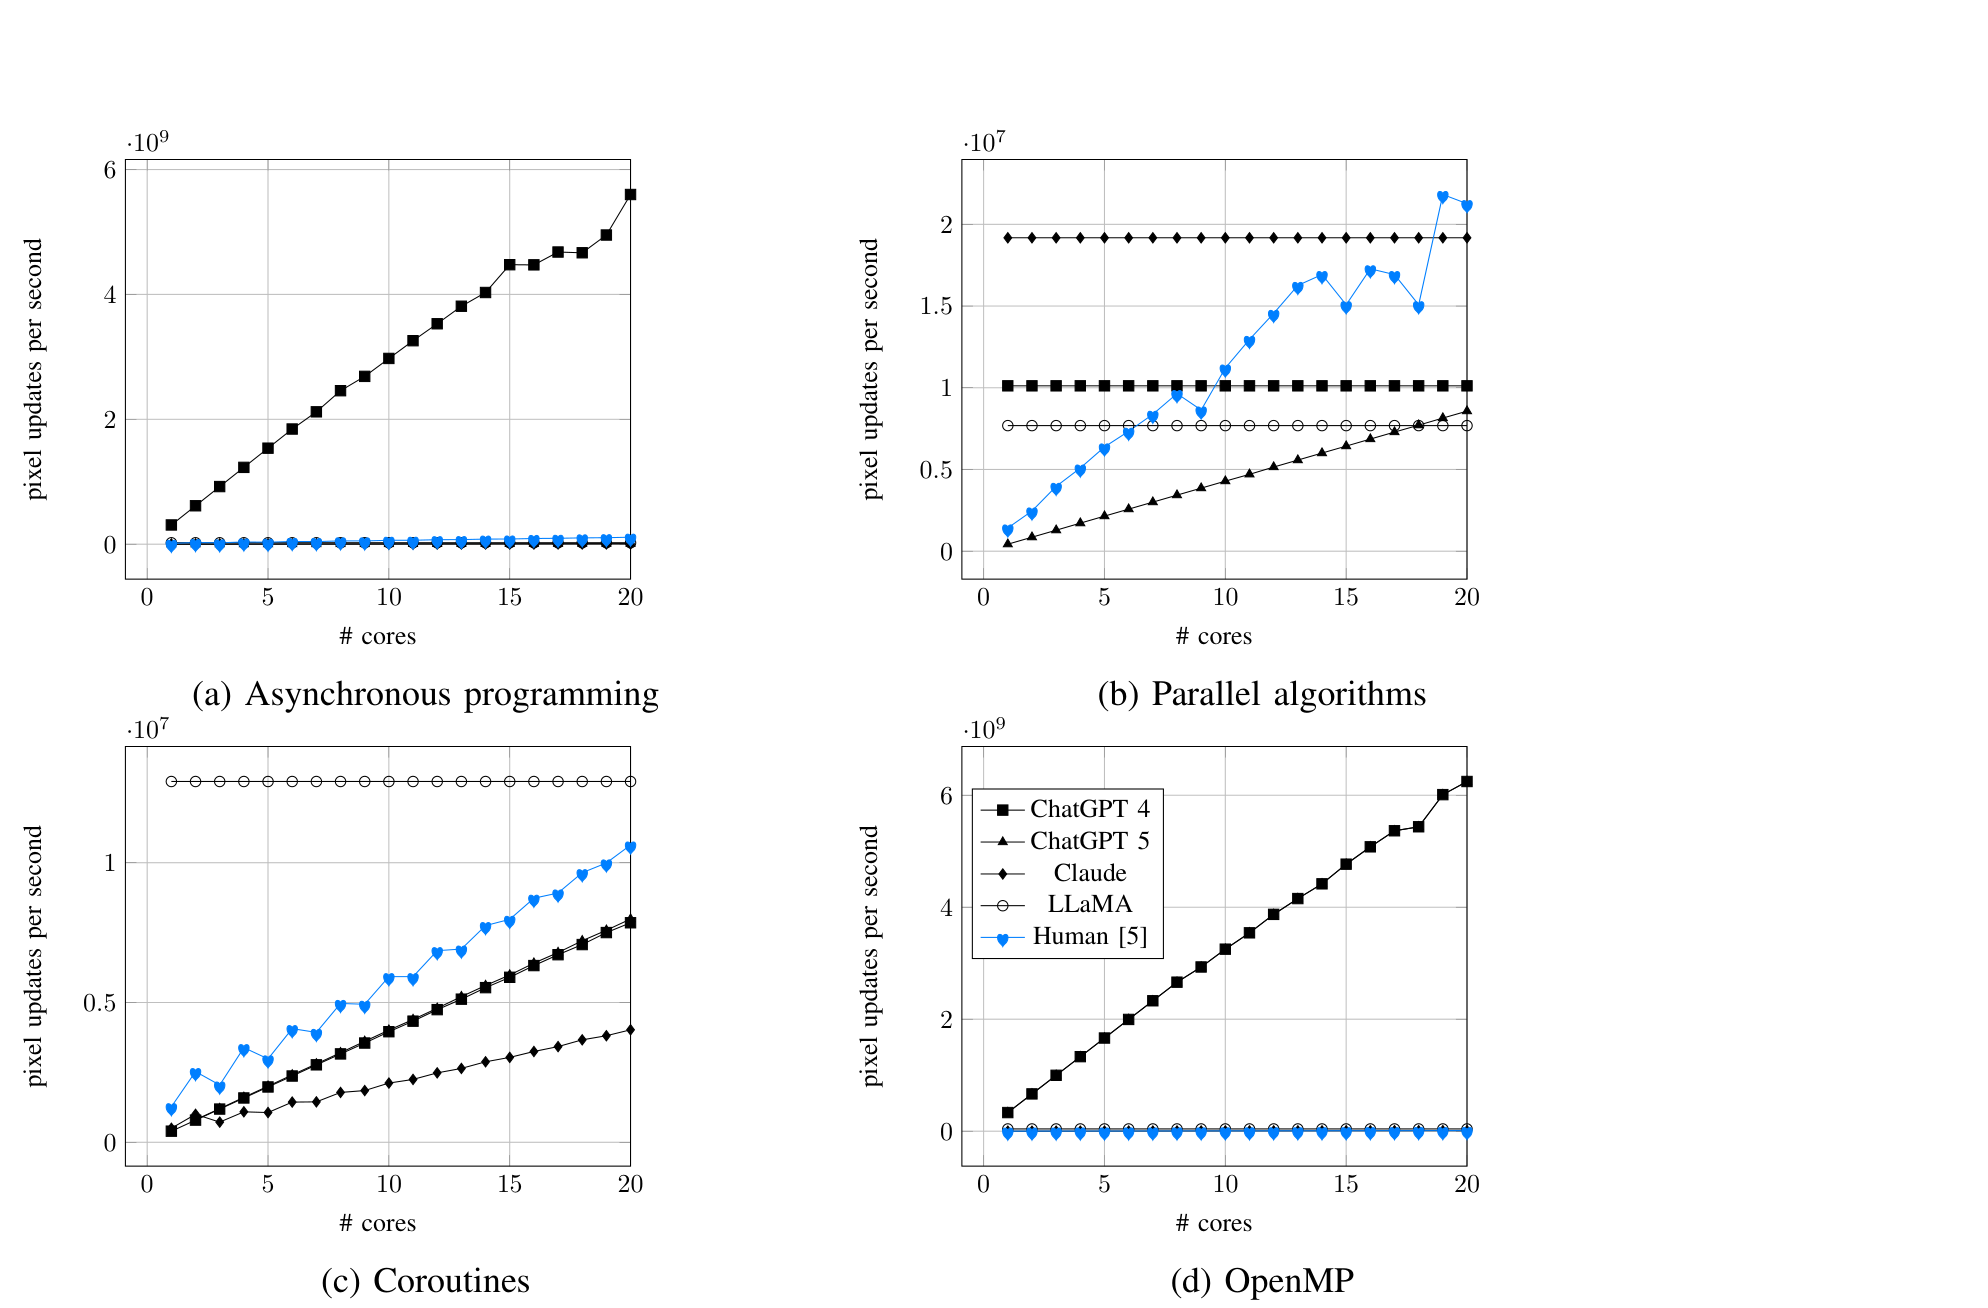
\includegraphics[width=0.95\textwidth]{figures/fig_scaling_shared.png}
\caption{Mở rộng trên một nút: (a) bất đồng bộ, (b) thuật toán song song,
(c) coroutine, (d) OpenMP. Nguồn: bài báo \cite{diehl2026}.}
\label{fig:scaling}
\end{figure}

\subsubsection{Bất đồng bộ}

ChatGPT-4 mở rộng gần tuyến tính đến 15 lõi; sau đó vẫn tăng nhưng chậm dần.
ChatGPT-5 và Claude cũng tăng đến 20 lõi, nhưng thông lượng tuyệt đối thấp hơn
một bậc độ lớn, nên trên thang tuyến tính với biên độ $6\times 10^9$ chúng bị ép
sát trục hoành trông như đường phẳng. LLaMA bỏ qua số luồng và luôn chạy trên toàn
bộ lõi. Điểm đáng chú ý là ChatGPT-4, dù mắc lỗi phân tích dòng lệnh, lại có phần
tính toán bất đồng bộ hiệu quả nhất trong nhóm LLM — cho thấy lỗi giao diện và
lỗi hiệu năng là hai chiều độc lập.

\subsubsection{Thuật toán song song}

ChatGPT-4 luôn dùng đủ 20 lõi bất kể tham số, nên đường biểu diễn là một đường
phẳng nằm ngang. ChatGPT-5 sửa được lỗi này và mở rộng đúng theo số lõi. Claude
và LLaMA cũng bỏ qua tham số số luồng. Đây là minh chứng rõ nhất cho luận điểm
“có tham số không có nghĩa là tôn trọng tham số”: cả bốn chương trình đều nhận
\code{-t}, nhưng chỉ một chương trình thực sự dùng nó để giới hạn backend.

\subsubsection{Coroutine}

ChatGPT-4 và ChatGPT-5 có đường mở rộng gần nhau. Claude cũng mở rộng nhưng chậm
hơn một chút. LLaMA không xét số lõi và nhanh hơn khi dùng toàn bộ lõi, nhưng
điều này không thể hiện khả năng mở rộng có kiểm soát. So với mã con người, cả
ba mô hình đều thấp hơn; đây là biến thể mà khoảng cách với chuyên gia lớn nhất.

\subsubsection{OpenMP}

ChatGPT-4 và ChatGPT-5 mở rộng tốt. Claude cũng mở rộng nhưng thông lượng thấp
hơn một bậc độ lớn, nên bị ép sát trục hoành trông như đường phẳng trên thang
tuyến tính. LLaMA chạy trên toàn bộ lõi và chậm hơn một bậc. Đáng chú ý, văn bản
bài báo gốc ghi nhận mã OpenMP của ChatGPT-5 vượt cả mã con người — một ngoại lệ
hiếm hoi mà LLM thắng ở cả tính đúng lẫn hiệu năng (tuy nhiên cần lưu ý rằng trên
đồ thị Hình~\ref{fig:scaling}d gốc, đường đạt $6\times 10^9$ lại mang ký hiệu ô
vuông của ChatGPT-4, nhiều khả năng là nhầm nhãn chuỗi dữ liệu khi vẽ hình).

\subsection{Khả năng mở rộng phân tán}

Với thí nghiệm phân tán, ảnh được đặt ở kích thước $12000\times80000$ điểm ảnh,
1000 vòng lặp. Mỗi nút chạy một rank MPI và 20 lõi OpenMP; mỗi rank tính một
phân vùng ảnh. Số nút được tăng theo cấp 1, 2, 4, 8, 12. Hình~\ref{fig:scalingdist}
trình bày kết quả trên thang logarit cơ số 2.

\begin{figure}[H]
\centering
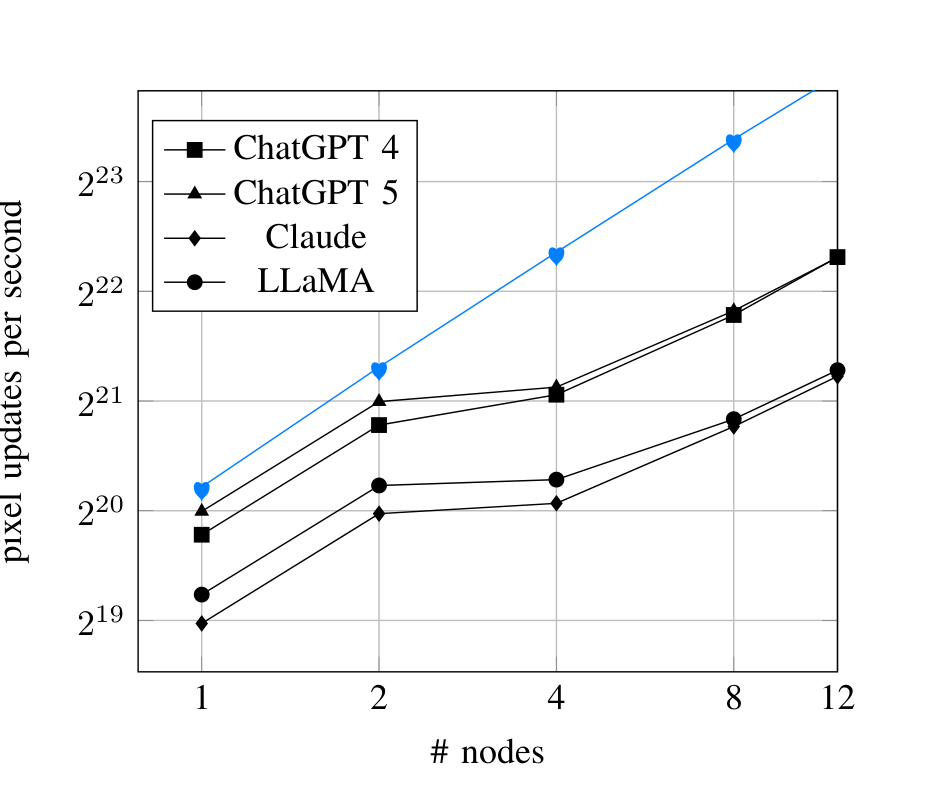
\includegraphics[width=0.62\textwidth]{figures/fig_scaling_dist.png}
\caption{Mở rộng phân tán từ 1 đến 12 nút (thang logarit cơ số 2; đường màu xanh
ký hiệu trái tim là mã con người tham chiếu từ \cite{diehl2024book}). Nguồn: bài
báo \cite{diehl2026}.}
\label{fig:scalingdist}
\end{figure}

Các quan sát chính:

\begin{itemize}
  \item ChatGPT-4 và ChatGPT-5 đều mở rộng, nhưng tăng tốc từ 2 lên 4 nút thấp
        hơn kỳ vọng; từ 8 lên 12 nút, hai mô hình có hiệu năng tương đương.
  \item Claude mở rộng nhưng chậm hơn hai mô hình OpenAI.
  \item LLaMA, sau khi sửa mốc đo thời gian, mở rộng và có hiệu năng tương đương
        Claude.
  \item Hiện tượng chững tăng tốc khi đi từ 2 lên 4 nút xuất hiện ở \emph{cả bốn}
        mã do LLM sinh, trong khi mã con người (đường màu xanh) vẫn tăng gần như
        đều đặn trên thang log--log. Một giả thuyết giải thích hợp lý về mặt toán
        học là do tập Mandelbrot đối xứng qua trục thực: chia tĩnh theo hàng thành
        2 nút tạo ra hai nửa trên/dưới có tải cân bằng tuyệt đối, nhưng sang 4 nút
        thì 2 dải giữa ôm gần hết tập Mandelbrot còn 2 dải rìa rất nhẹ, khiến nút
        chậm nhất chặn toàn hệ thống trước bước gom dữ liệu.
  \item Mã con người vẫn dẫn đầu trên toàn dải số nút. Tác giả cho rằng cần phân
        tích sâu hơn các mẫu truyền thông và phân vùng để giải thích đầy đủ khoảng
        cách này.
\end{itemize}

Điểm đáng khích lệ là sau khi sửa một số lỗi thực thi, \emph{mọi} mã đều mở rộng
được. Điều này cho thấy LLM có thể tạo ra cấu trúc phân tán đúng ở mức khung
(phân vùng, gom dữ liệu, ghi ảnh), ngay cả khi chi tiết biên còn sai. Điểm cần
thận trọng là kết quả chỉ đo một lần cho mỗi cấu hình, nên các chênh lệch nhỏ
giữa các đường cong không nên được diễn giải quá mức.

\subsection{So sánh với mã con người}

Bảng~\ref{tab:human} tóm tắt so sánh giữa mã LLM và mã trong sách
\emph{Parallel C++} \cite{diehl2024book}. Việc chọn mã sách — đã tối ưu nhưng
không tối ưu cực đoan — nhằm tạo một mốc so sánh công bằng, không phải một đối
thủ được huấn luyện riêng cho benchmark.

\begin{table}[H]
\centering
\small
\caption{So sánh tương đối giữa mã LLM và mã con người theo từng biến thể.}
\label{tab:human}
\begin{tabularx}{\textwidth}{@{}p{3.2cm} X p{3.3cm}@{}}
\toprule
\textbf{Biến thể} & \textbf{Kết quả so sánh} & \textbf{Nhận xét} \\
\midrule
Bất đồng bộ & ChatGPT-4 nhanh hơn mã sách nhờ thêm tối ưu & LLM có thể vượt ở mẫu đơn giản \\
Thuật toán song song & Mã sách nhanh hơn ChatGPT-5 & Mã sách mở rộng tốt hơn \\
Coroutine & Mã sách nhanh hơn ChatGPT-4/5 và Claude & Khoảng cách lớn nhất \\
OpenMP & ChatGPT-5 nhanh hơn cả mã sách (theo văn bản gốc; xem lưu ý Hình~\ref{fig:scaling}d) & Ngoại lệ nổi bật \\
MPI+OpenMP & Mã sách nhanh hơn mọi mã LLM & Cần phân tích truyền thông sâu hơn \\
\bottomrule
\end{tabularx}
\end{table}

Bức tranh tổng thể không đồng nhất. Ở các mẫu đơn giản (async, OpenMP), LLM có
thể ngang hoặc vượt mã sách. Ở các mẫu đòi hỏi điều phối tinh vi (coroutine,
MPI), mã con người vẫn tốt hơn. Điều này phù hợp với giả thuyết rằng LLM mạnh ở
việc tái sử dụng mẫu phổ biến, nhưng yếu ở việc suy luận về vòng đời tài nguyên
và chi phí truyền thông trong một ngữ cảnh cụ thể.
